%\renewcommand{\thefootnote}{\arabic{footnote}}
\chapter{TINJAUAN PUSTAKA}
\label{BAB2:tinjauan}
\section{Transformator Daya}

Transformator daya merupakan salah satu peralatan tenaga listrik yang berfungsi dalam mentrasmisikan daya listrik dengan cara menaikkan dan menurunkan tegangan  listrik \cite{sutaryono2015analisa}. Hal ini bertujuan dalam mengurangi rugi-rugi daya yang dikarenakan adanya impedansi yang timbul akibat jarak transmisi yang panjang dapat dikurangi dengan menaikkan tegangan. Transformator daya ditempatkan pada sisi pembangkitan untuk menaikkan tegangan dan pada sisi penerimaan untuk menurunkan tegangan. Merujuk pada standar PLN 61 : 1997 pengelompokan transformator yakni berdasarkan tegangan operasinya yang melebihi 20 kV \cite{sutaryono2015analisa}. Karena beroperasi pada daya dan tegangan tinggi maka diperlukan sistem pengaman pada transformator daya sehingga dapat bekerja dengan aman dan terhindar dari adanya gangguan sistem tenaga listrik. Sistem pengaman pada transformator daya ialah dengan menggunakan bahan dielektrik cair yakni minyak transformator serta berupa dielektrik pada berupa kertas . Selain dalam menahan tegangan yang tinggi adanya minyak transformator juga berfungsi dalam menghantarkan panas dari dalam akibat rugi-rugi daya ke udara bebas sehingga panas berlebih dapat dicegah \cite{krause2012power}.



%\begin{equation}
%  L(x,W)= \frac{1}{N}\sum\limits_{i=0}^{N} l(x_i,W)   
%  \label{func:loss}
%\end{equation}

\section{Indeks Kesehatan Trafo}
Dalam sistem jaringan tenaga listrik pada umumnya transformator daya yang digunakan saat beroperasi yang memiliki kondisi yang baik agar terhindar dari gangguan. Kondisi sebuah transformator secara keseluruhan dapat dievaluasi dengan sebuah metode yakni indeks kesehatan transformator \cite{nurcahyanto2019analysis}. Metode ini merupakan hasil kombinasi data hasil inspeksi lapangan, selama beroperasi maupun hasil pengujian transformator daya di laboratorium atau lapangan \cite{ortiz2016health}. Pengujian pada transformator daya dibagi atas pengujian elektrik, pengujian kimia, dan pengujian fisik. Metode-metode yang sering digunakan pada transformator daya diantaranya adalah \textit{Dissolve Gas Analysis} (DGA), kualitas minyak transformator, furan, faktor daya, pemantauan \textit{tap changer}, riwayat pembebanan serta data pemeliharaan \cite{jahromi2009approach}.

\subsection{\textit{Dissolve Gas Analysis} (DGA)}
DGA merupakan salah satu metode yang digunakan dalam mendeteksi adanya gangguan pada transformator daya. Dalam kondisi normal dielektrik cair pada transformator daya tidak mengalami dekomposisi dengan cepat. Namun jika terjadi adanya gangguan termal atau elektrik dapat mempercepat laju dekomposisi pada dielektrik. Proses dekomposisi dapat menghasilkan gas kontaminan yang dapat mengubah sifat kondutivitas dari isolator yang dapat memicu adanya gangguan lanjutan. Secara umum terdapat beberapa jenis gas hasil dekomposisi yang dilakukan pengecekan diantaranya adalah hidrogen (H$_2$), metana (CH$_4$), asetilen (C$_2$H$_2$), etilen (C$_2$H$_4$), etana (C$_2$H$_6$), selain itu bahan dielektrik pada berupa kertas juga mengalami dekomposisi yang menghasilkan karbon monoksida (CO) dan karbon dioksida (CO$_2$) \cite{ahmed2013power}. Beberapa dari konsentrasi masing-masing gas yang telah diketahui kemudian dapat dianalisis dengan menggunakan segitiga Duval\cite{duval1989dissolved}. Hal dapat dilihat pada Gambar \ref{gambar:duval triangle} untuk menentukan jenis gangguan yang terjadi, yang terdiri dari:

\begin{itemize}
	\item[] a. Percikan energi tinggi (\textit{High-energy Arching})
	\item[] b. Percikan energi rendah (\textit{Low-energy Arching})
	\item[] c. Peluahan korona (\textit{Corona Discharges})
	\item[] d. Titik panas suhu rendah (\textit{Hot spots}, T $<$ 200$^{\circ}$C)
	\item[] e. Titik panas suhu sedang (\textit{Hot spots},200$^{\circ}$C $<$ T $<$ 400$^{\circ}$C)
	\item[] f. Titik panas suhu tinggi (\textit{Hot spots}, T $>$ 400$^{\circ}$C)
\end{itemize}

\begin{figure}[h]
	\begin{center}
    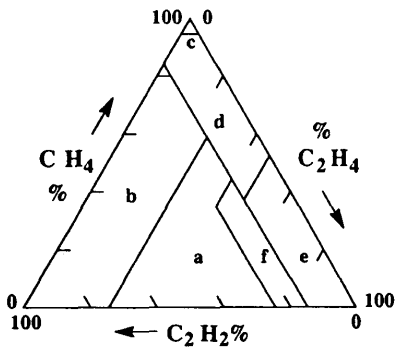
\includegraphics[width=0.5\textwidth]{BAB-2/figures/duval triangle.png}	
	    \caption{Segitiga Duval \cite{duval1989dissolved}}
	    \label{gambar:duval triangle}
	\end{center}
\end{figure}

\subsection{Kualitas Minyak Transformator}
Pada sebuah transformator daya peranan minyak adalah sebagai isolator cair, penghantar panas ke udara luar serta pelindung bagian dalam. Adapun fungsi sebagai isolator cair adalah untuk mencegah adanya loncatan listrik keluar karena pada umumnya transformator daya beroperasi pada tegangan tinggi. Kegunaan minyak transformator sebagai penghantar panas adalah untuk menjaga kestabilan suhu transformator karena adanya rugi-rugi daya yang berubah menjadi kalor. Sedangkan sebagai pelindung adalah untuk mencegah adanya reaksi kimia dari logam bagian dalam terhadap oksigen yang dapat menyebabkan adanya korosi \cite{pln2003panduan}.

Minyak transformator daya dapat beroperasi dengan baik jika belum melampaui batasan-batasan standar yang ditetapkan di antaranya tingkat keasaman serta kandungan airnya yang dapat diketahui melalui pengujian secara kimia \cite{ieee2007ieee}. Selain itu pengujian secara fisik dapat diperoleh \textit{interfacial tension} yang menjadi indikator banyaknya kontaminan polar tang terlarut dalam minyak \cite{sutaryono2015analisa}. Adapun pengujian elektrik dapat membantu mengetahui batas ambang tegangan yang dapat ditahan oleh bahan dielektrik transformator daya, hal ini dengan tegangan tembus (\textit{breakdown voltage}). Semakin tinggi nilai dari tegangan tembusnya maka semakin aman suatu transformator daya untuk dioperasikan. Tegangan tembus terjadi karena adanya elektron bebas pada bahan dielektrik, adanya elektron bebas pada bahan dielektrik disebabkan keberadaan kontaminan baik berupa gas, cair maupun padat pada sistem isolasi. Standar yang dijadikan rujukan untuk mengetahui kondisi minyak transformator adalah IEC 60422-2013 \cite{standard2013mineral}.

\begin{table}[h]
	\centering
	\caption{Standar Pengujian Minyak Tranformator}
	\label{tabel:standar minyak}
	\begin{tabular}{|c|c|c|c|c|c|} 
		\hline
		\multirow{2}{*}{\textbf{Parameter Uji}}                                                                 & \multirow{2}{*}{\textbf{Metode}}                   & \multicolumn{3}{c|}{\textbf{\textit{Score }(Si) batas IEC 60422:2013}} & \multirow{2}{*}{\begin{tabular}[c]{@{}c@{}}\textbf{Weight}\\~(Wi)\end{tabular}}  \\ 
		\cline{3-5}
		&                                                    & \textit{Good}(1) & \textit{Fair (2)} & Poor (3)                        &                                                                                  \\ 
		\hline
		\begin{tabular}[c]{@{}c@{}}\textbf{Tegangan Tembus}\\\textbf{(kV/2.5mm)}\end{tabular}                   & IEC 156                                            &  50              & 40 - 50           &  40                             & 3                                                                                \\ 
		\hline
		\begin{tabular}[c]{@{}c@{}}\textbf{Kandungan Air}\\\textbf{(mg/kg)}\end{tabular}                        & \begin{tabular}[c]{@{}c@{}}IEC\\60814\end{tabular} &  20              & 20 - 30           &  30                             & 4                                                                                \\ 
		\hline
		\begin{tabular}[c]{@{}c@{}}\textbf{Keasaman}\\\textbf{(mgKOH/g)}\end{tabular}                           & C2011K06                                           &  0.1             & 0.15 - 0.2        &  0.2                            & 1                                                                                \\ 
		\hline
		\begin{tabular}[c]{@{}c@{}}\textit{\textbf{Interfacial Tension}}\\\textit{\textbf{(mN/m)}}\end{tabular} & ISO 6295                                           &  28              & 22 - 28           &  22                             & 2                                                                                \\
		\hline
	\end{tabular}
\end{table}

\subsection{Pengujian Furan}
Seiring menurunnya umur dari minyak transformator daya akan membentuk suatu senyawa kimia yang dikenal dengan furan. Pembentukan furan juga disebabkan adanya suhu yang tinggi serta proses oksidasi senyawa asam. kerusakan akibat peningkatan konsentrasi di udara serta keberadaan oksigen dapat meningkatkan proses pembentukan furan. Keberadaan furan dapat menjadi acuan mengenai umur dari dielektrik padat yang berupa kertas. Standar pengujian furan disajikan pada Tabel \ref{tabel:standar furan} \cite{sutaryono2015analisa}.

\begin{table}[h]
	\centering
	\caption{Standar Pengujian Furan}
	\label{tabel:standar furan}
	\begin{tabular}{|c|c|c|c|} 
		\hline
		\textbf{No} & \begin{tabular}[c]{@{}c@{}}\textbf{2 FAL saat 55$^{\circ}$C }\\\textbf{(ppb)}\end{tabular} & \begin{tabular}[c]{@{}c@{}}\textbf{Estimasi }\\\textbf{~Umur Kertas (\%)}\end{tabular} & \textbf{Keterangan}                                          \\ 
		\hline
		1           & 58                                                                               & 100                                                                                    & \multirow{3}{*}{Penuaan Normal}                       \\ 
		\cline{1-3}
		2           & 130                                                                              & 90                                                                                     &                                                              \\ 
		\cline{1-3}
		3           & 292                                                                              & 79                                                                                     &                                                              \\ 
		\hline
		4           & 654                                                                              & 66                                                                                     & \multirow{4}{*}{Percepatan Penuaan}                   \\ 
		\cline{1-3}
		5           & 1464                                                                             & 50                                                                                     &                                                              \\ 
		\cline{1-3}
		6           & 1720                                                                             & 46                                                                                     &                                                              \\ 
		\cline{1-3}
		7           & 2021                                                                             & 42                                                                                     &                                                              \\ 
		\hline
		8           & 2374                                                                             & 38                                                                                     & \multirow{3}{*}{Daerah Peringatan : Penuaan Tidak Normal}  \\ 
		\cline{1-3}
		9           & 2789                                                                             & 33                                                                                     &                                                              \\ 
		\cline{1-3}
		10          & 3277                                                                             & 29                                                                                     &                                                              \\ 
		\hline
		11          & 3851                                                                             & 24                                                                                     & \multirow{2}{*}{Sangat Rentan Gangguan}             \\ 
		\cline{1-3}
		12          & 4524                                                                             & 19                                                                                     &                                                              \\ 
		\hline
		13          & 5315                                                                             & 13                                                                                     & \multirow{3}{*}{Akhir Pemakaian Kertas}                   \\ 
		\cline{1-3}
		14          & 6245                                                                             & 7                                                                                      &                                                              \\ 
		\cline{1-3}
		15          & 7337                                                                             & 0                                                                                      &                                                              \\
		\hline
	\end{tabular}
\end{table}



%Furan adalah senyawa organik yang terbentuk karena penurunan
%nilai minyak isolasi, panas berlebih, dan oksidasi asam. Kerusakan yang
%disebabkan oleh kelembaban ditambah dengan oksigen mempercepat
%penghancuran isolasi dan membentuk senyawa furan. Kandungan furan
%pada minyak sangat menentukan sisa usia dari kertas isolasi. Estimasi
%umur kertas isolasi berdasarkan jumlah konsentrasi furan yang ada di
%dalam minyak isolasi ditampilkan pada Tabel 2.3.




\section{\textit{Machine Learning}}
Machine learning merupakan salah satu metode yang digunakan dalam mempelajari pola serangkaian data dengan proses komputasi digital \cite{jordan2015machine}. Secara sederhana algoritma dirancang untuk digunakan dalam mempelajari suatu data kemudian dapat melakukan prediksi berdasarkan \textit{input} baru yang diberikan. Berdasarkan cara belajarnya terdapat pengelompokkan pada \textit{machine learning} yakni \textit{supervised learning} dan \textit{unsupervised learning} . Pada \textit{supervised learning} model dapat mempelajari data yang memiliki fitur yang dilengkapi dengan data target, sedangkan pada \textit{unsupervised learning} model belajar tanpa menggunakan adanya data target sehingga pada proses prediksi model akan memberikan keluaran berupa pengelompokan data \cite{alpaydin2020introduction}.

\textit{Machine Learning} telah mengalami banyak modifikasi untuk menyesuaikan jenis data yang diolah.  Arsitektur baru dari \textit{machine learning} yang banyak digunakan saat ini berupa algoritma yang meniru sistem kerja syaraf manusia yang dikenal dengan algoritma \textit{Artificial Neural Network} (ANN) \cite{braspenning1995artificial}. Dengan menggunakan ANN sistem memungkinkan dalam mengenali objek dalam sebuah gambar merupakan salah satu implementasinya. Adapun pada pengolahan data yang bersifat \textit{time series} atau berupa deret ANN dikembangkan agar dapat melakukan sebuah prediksi berdasarkan \textit{input} yang diterima sebelumnya sebagai dasar referensi prediksi ke depan. Model tersebut dikenal dengan \textit{Recurrent Neural Network} dimana setiap \textit{input} yang diterima sebelum dilakukan prediksi akan diproses secara berulang pada satu sel RNN sehingga model dapat mengingat informasi pentingnya \cite{medsker2001recurrent}.


\section{\textit{Long Short Term Memory (LSTM)}}
Pada pemodelan dengan menggunakan metode RNN secara umum memiliki kemampuan dalam membuat prediksi yang dipengaruhi oleh \textit{input} sebelumnya. Namun terdapat kekurangan pada metode tersebut yakni tidak mampu mengatasi dengan  seri yang panjang, misalnya pada sebuah data \textit{time series}, RNN akan sulit mengkorelasikan antara data saat ini dengan data yang sangat lampau, akibatnya jika data yang diproses dalam rentang waktu yang lama maka RNN hanya mampu membuat prediksi yang hanya berkaitan pada waktu yang pendek. Kekurangan pada RNN dikarenakan adanya \textit{vanising gradient}, yakni menghapus data yang tidak berkaitan dengan data baru yang dimasukkan. Adanya kekurangan tersebut maka dibutuhkan suatu metode baru yang dapat mengingat data lampau saat menerima \textit{input} terbaru. 
LSTM merupakan salah satu turunan dari pemodelan matematis yang digunakan dalam mengenali pola serangkaian data 

Kelebihan yang dimiliki LSTM dibandingkan dengan RNN dikarenakan algoritma yang digunakan terdiri dari struktur yang kompleks. Secara umum terdapat 4 bagian pada arsitektur LSTM yakni \textit{forget gate}, \textit{input gate}, \textit{Cell gate}, dan \textit{Output gate}. 
\subsection{\textit{Forget Gate}}
Pada \textit{Forget gate} merupakan bagian yang menentukan mengenai informasi pada keluaran sel sebelumnya untuk dipertahankan atau dihapus. Hal ini dilakukan dengan memasukkan keluaran sel sebelumnya yang digabungkan dengan masukan baru ke dalam fungsi aktivasi sigmoid. Informasi akan dipertahankan untuk hasil dari sigmoid dengan nilai 1 dan dihapus untuk keluaran yang bernilai 0. Secara matematis pada \textit{forget gate} digunakan persamaan sebagai berikut:
\begin{equation}
	\boldsymbol{f_t} = \sigma_g(\boldsymbol{W_{f}}.[\boldsymbol{h_{t-1}}, \boldsymbol{x_t}] + \boldsymbol{b_f})
	\label{func:forget}
\end{equation} 
Berdasarkan persamaan~(\ref{func:forget}) dapat diketahui pada persamaan tersebut terdapat bentuk $[\boldsymbol{h_{t-1}}, \boldsymbol{x_t}]$. Hal ini merupakan operasi penggabungan vektor yakni penggabungan baris pada $\boldsymbol{h_{t-1}}$ dengan baris pada $\boldsymbol{x_t}$.
\subsection{\textit{Input Gate}}
Salah satu kelebihan LSTM adalah dapat mengingat informasi data masukan yang lama. Hal ini dikarenakan karena adanya satu bagian yang berperan dalam memperbarui memori berdasarkan informasi penting dari masukan baru. Kemampuan ini diperoleh karena ada dua tahapan penting pada \textit{input gate} yakni melalui lapisan \textit{sigmoid} dan \textit{tanh}. lapisan akan memberikan keluaran berupa nilai mana saja yang harus dilakukan pembaruan pada memori sedangkan lapisan \textit{tanh} memberikan keluaran berupa calon ($\boldsymbol{\tilde{C}}$) yang ditambahkan pada memori. 
\begin{equation}
	\boldsymbol{i_t} = \sigma_i(\boldsymbol{W_{f}}.[\boldsymbol{h_{t-1}}, \boldsymbol{x_t}] + \boldsymbol{b_i})\\
	\label{func:input}
\end{equation}
\begin{equation}
	\boldsymbol{\tilde{C}} = tanh(\boldsymbol{W_{C}}.[\boldsymbol{h_{t-1}}, \boldsymbol{x_t}] + \boldsymbol{b_C})
	\label{func:C-tilde}
\end{equation}
Hasil perkalian dari dua lapisan pada \textit{input gate} akan menjadi \textit{input} pada memori sebagai pembaruan. pembaruan yang terjadi dalam hanya dalam jumlah yang sedikit, oleh karena itu informasi penting pada data yang lampau akan tetap tersimpan untuk jumlah data yang banyak.
\subsection{\textit{Cell gate}}
\textit{Cell gate} merupakan tempat penyimpanan informasi penting pada setiap data yang diberikan pada LSTM. \textit{cell gate} terdiri dari masukan dari \textit{forget gate} untuk mengurangi informasi yang tidak diperlukan dari semua masukan sebelumnya melalui persamaan ~(\ref{func:forget}). Kemudian ditambahkan dengan hasil perkalian dari $\boldsymbol{i_t}$ dan $\boldsymbol{\tilde{C}}$.
\begin{equation}
	\boldsymbol{C_t} = \boldsymbol{f_t}*\boldsymbol{C_{t-1}} + \boldsymbol{i_t} * \boldsymbol{\tilde{C}}
	\label{func:cell_gate}
\end{equation}
Hal utama yang perlu diperhatikan adalah bahwa pada LSTM bagian \textit{cell gate} merupakan lapisan yang saling terhubung, sehingga antar sel yang berjauhan pun dapat terintegrasi. Kondisi ini yang menjadikan LSTM dapat mengatasi permasalahan versi RNN sebelumnya yang diakibatkan adanya \textit{vanishing gradient}.
\subsection{\textit{Output Gate}}
Pada bagian akhir merupakan keluaran dari sel lstm atau dapat berupa hasil prediksi berdasarkan masukan yang diberikan. Keluaran ditentukan oleh memori $\boldsymbol{C_t}$ dan masukan yang diberikan. Hal ini dilakukan dengan memasukkan  $\boldsymbol{x_t}$ dan keluaran sebelumnya ($\boldsymbol{h_{t-1}}$) pada fungsi \textit{sigmoid}. Hasil dari fungsi \textit{sigmoid} kemudian akan memfilter nilai dari \textit{cell state} yang dapat diteruskan menuju keluaran. Sebelum dikalikan dengan hasil dari gerbang \textit{sigmoid}, \textit{cell state} terlebih dahulu melewati gerbang tanh untuk mengubah nilai pada rentang -1 sampai 1. Secara matematis dapat dituliskan sebagai berikut:
\begin{equation}
	\boldsymbol{o_t} = \sigma(\boldsymbol{W_i}.[\boldsymbol{h_{t-1}}, \boldsymbol{x_t}] + \boldsymbol{b_o})
	\label{func:ouput_sigmoid}
\end{equation}
\begin{equation}
	\boldsymbol{h_t} = \boldsymbol{o_t}*tanh(\boldsymbol{C_t})
	\label{func:final_output}
\end{equation}

%Informasi ini diperoleh pada lapisan sebelumnya yakni kombinasi dari \textit{forget gate} dan \textit{input gate}. Pada dasarnya 

%\begin{align}
%	f_t &= \sigma_g(W_{f} x_t + U_{f} c_{t-1} + b_f) \\
%	i_t &= \sigma_g(W_{i} x_t + U_{i} c_{t-1} + b_i) \\
%	o_t &= \sigma_g(W_{o} x_t + U_{o} c_{t-1} + b_o) \\
%	c_t &= f_t \circ c_{t-1} + i_t \circ \sigma_c(W_{c} x_t + b_c) \\
%	h_t &= o_t \circ \sigma_h(c_t)
%\end{align}
%\lipsum[5-6]
%\begin{table}[h]
%    \centering
%    \caption{Rata-rata loss dan accuracy Model A untuk seluruh round}
%\begin{tabularx}{0.95\textwidth} { 
%  | >{\centering\arraybackslash}X 
%  | >{\centering\arraybackslash}X | }
% \hline
%  train\_accuracy &	0.46846 \\
% \hline
%  train\_loss &	2.71451 \\
% \hline
%  val\_accuracy &	0.47391 \\
%  \hline
%  val\_loss & 2.69424 \\
%  \hline
%\end{tabularx}
%    \label{tab:my_label} 
%\end{table}
%
%\lipsum[7]
%\begin{center}
%\begin{figure}[h]
%    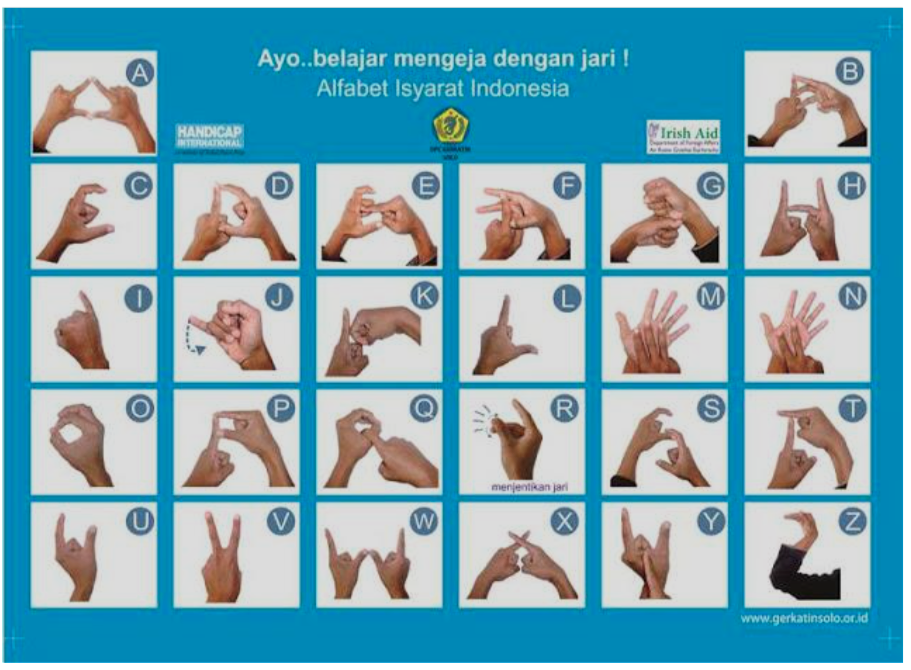
\includegraphics[width=\textwidth]{BAB-2/figures/alfabetbisindo.png}	
%	    \caption{Alfabet Bisindo (Almuharram, 2013).}
%	    \label{gambar:alfabet bisindo}
%\end{figure}
%\end{center}
%Gambar \ref{gambar:alfabet bisindo} menyunjukkan sudut pandang umum yang digunakan dalam berkomunikasi menggunakan bahasa isyarat, yaitu tampak depan \citep{xiong2004_dscForSensorNetworks}. Sehingga, data gambar yang digunakan di penelitian ini juga memuat gestur Bisindo dari tampak depan, dengan persamaan~(\ref{func:loss}), dengan hasil penelitian di Bab~\ref{BAB4:hasil}.